\section{Разработка учебного материала для курса ТиМП}
\pretolerance10000

Достаточно очевидным является тот факт, \hfilчто \hfilстуденты, \hfilзанимающиеся \\программированием, \hfilобучаясь\hfil на\hfil специальности\hfil \hfil<<Информационная\hfil\\ безопасность>>, должны уметь разрабатывать свои программы, не допуская каких-либо уязвимостей в своем коде. Вполне логично было бы обучать студентов аспектам безопасности программирования на предмете <<Технологии и методы программирования>> (ТиМП). К сожалению, текущий курс ТиМП не охватывает подобные проблемы, поэтому было принято решение о том, что он нуждается в развитии.\par 
Платформа FHQ включает в себя специальную систему Classbook, позволяющую хранить и предоставлять учебную информацию. Эта система поможет обучить студентов основным существующим уязвимостям, встречающимся в программном обеспечении, и поможет им избегать их при разработке собственных приложений.\par 
Также FHQ послужит площадкой для выполнения практических заданий по темам, связанным с уязвимостями программного обеспечения, и позволит на практике закрепить полученные в ходе прохождения курса знания.\par
В качестве темы для первых тестовых лекции и практического занятия была выбрана уязвимость <<Переполнение стека>>. Ее подтверждает тот факт, что уязвимости, относящиеся к переполнению различных сегментов памяти, обнаруживаются специалистами регулярно. Проиллюстрировать этот довод могут две уязвимости, включенные в реестр CVE (Common Vulnerabilities and Exposures – список общих уязвимостей, подверженных воздействиям извне) за последнее время, а именно CVE-2015-7547 [7] и CVE-2018-10731 [8].
\vspace{\baselineskip}

\subsection{Формирование лекции для курса ТиМП}
Для подготовки материала к новой лекции курса ТиМП была взята и переработана информация с англоязычного ресурса Техасской группы технической безопасности RaiderSec [9].\par
Для демонстрации уязвимости, связанной с переполнением стека, используется программа третьего уровня игры <<Smash The Stack -- IO>> [10], призванной показать на практике механизмы работы уязвимостей. Исходный код программы представлен на рисунке 14.\par
\begin{center}
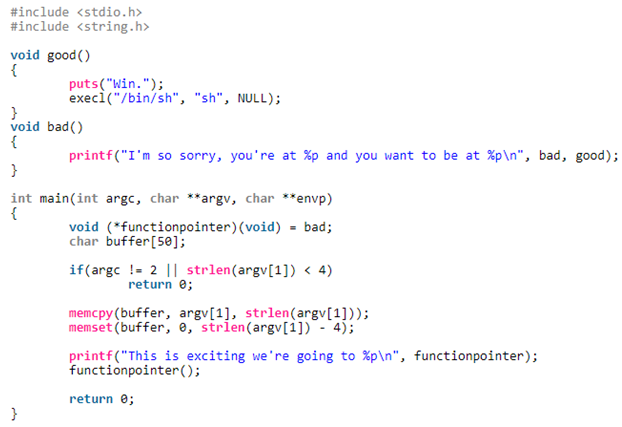
\includegraphics[width=0.65\textwidth]{13}\\
Рисунок 14 -- Исходный код программы, демонстрирующей уязвимость\\
\end{center}
\vspace{\baselineskip}

Допустим, злоумышленнику интересен некий абстрактный флаг, скрытый в программе в функции good. Суть экслойта (программы или кода, использующего уязвимость с целью извлечения выгоды) заключается в том, что при передаче в буфер более 50 символов произойдет его переполнение, и часть данных перезапишется поверх адреса функции bad.\par 
Таким образом, возникает возможность изменить адрес функции, и, когда код продолжит свое исполнение, в месте предполагаемого вызова функции bad будет вызвана функция good, следовательно, злоумышленник получит доступ к секретным данным.\par
Чтобы наглядно продемонстрировать расположение функций и их аргументов в адресном пространстве памяти, код программы был дизассемблирован посредством отладчика GDB. Далее на основе полученных данных было составлено схематическое расположение функций и их аргументов по конкретным адресам в различных сегментах памяти на протяжении всего времени работы программы (рис. 15).\par
\begin{center}
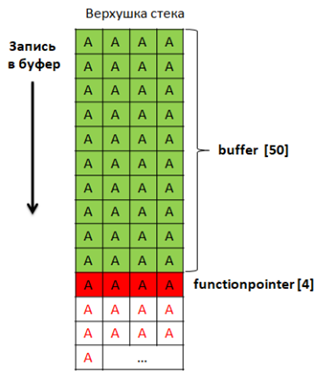
\includegraphics[width=0.65\textwidth]{14}\\
Рисунок 15 -- Схематичное представление памяти стека\\
\end{center}
\vspace{\baselineskip}

На основе полученных данных было разработано краткое методическое пособие, подробно описывающее на низком уровне работу программы задачки <<Smash The Stack -- IO>>. Дополнительно была оформлена презентация, содержащая наглядную демонстрацию отладки программы с использованием GDB с комментариями.\par
В скором времени методическое пособие, а также презентация будут загружены в ресурс FHQ в систему Classbook для доступа студентов и всех желающих.\par
\vspace{\baselineskip}

\subsection{Разработка практического задания для FHQ}
Для того, чтобы обучающиеся на курсе ТиМП студенты могли на практике закрепить знания, полученные в ходе изучения была разработана программа, содержащая в себе уязвимость переполнения стека. Код программы представлен на рисунке 16.\par
\begin{center}
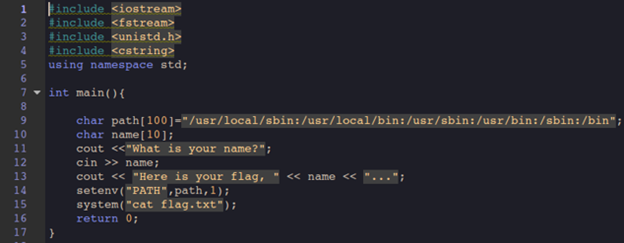
\includegraphics[width=0.65\textwidth]{15}\\
Рисунок 16 -- Исходный код программы для практического задания\\
\end{center}
\vspace{\baselineskip}

Данная программа базируется на принципах, схожих с принципами, описанными в методическом пособии и презентации, и также повержена уязвимости переполнения стека.\par 
В скором времени на платформе FHQ появится новый раздел, в который будет помещена данная программа, и студенты или каждый желающий смогут проверить свои знания и попытаться заполучить скрытый флаг.\par
\clearpage